\chapter{Fundamentação Teórica}
\label{fund_teo}
% ----------------------------------------------------------

\section{Python}

Python é uma linguagem de programação de alto nível, orientada a objetos e interpretada \cite{van1995python}. Possui uma presença muito forte nos meios acadêmicos e profissionais devido a sua filosofia de priorizar o esforço do programador sobre o esforço da máquina. Em outras palavras, Python é conhecido por sua fácil leitura, aprendizado e rapidez de desenvolvimento de aplicações, além de possuir código aberto e conexões com os mais diversos módulos e \textit{frameworks}.

A linguagem é talvez a mais utilizada no campo de ciência da informação pois, além dos motivos já mencionados, possui diversos módulos de visualização de dados e que, somados à facilidade de leitura do código, proporciona uma visão clara dos dados, até para os não iniciados. Dessa forma, a linguagem é excelente para o desenvolvimento de aplicações de aprendizado de máquina, graças à facilidade da manipulação e visualização de dados e estatísticas e da alta integração com bibliotecas de desenvolvimento de modelos de inteligência artificial.

\section{Scikit-Learn}

Uma biblioteca para Python muito conhecida na área de ciência de dados e de aprendizado de máquinas \cite{sklearn_api}. O projeto de código aberto vem desenvolvendo algoritmos desde 2010, focando na manipulação e tratamento de dados, assim como no desenvolvimento de algoritmos de aprendizado de máquina \cite{scikit-learn}.

O scikit-learn é uma ferramenta valiosa para cientistas de dados, engenheiros de aprendizado de máquina e pesquisadores que desejam explorar e aplicar técnicas de aprendizado de máquina e mineração de dados em seus projetos. Ele permite que os usuários construam, avaliem e ajustem modelos de \textit{machine learning} de maneira eficaz e eficiente, tornando-o uma escolha popular no campo do processamento de dados e aprendizado de máquina.

% \section{Tensorflow 2.0 \& Keras}
% %\todo{PYTORCH}
% Tensorflow 2.0 é uma plataforma de desenvolvimento de algoritmos de aprendizado de máquina em python. No mercado atual, é utilizado amplamente por grandes empresas devido a sua robustez e flexibilidade.  A plataforma é adequada ao uso por profissionais ou amadores, oferecendo um ecossistema capaz de satisfazer as necessidades de ambos \cite{tensorflow2015-whitepaper}.

% Dentro do ecossistema mencionado, existe o módulo Keras. Esta biblioteca providencia uma interface de alto nível para o desenvolvimento de aplicações de aprendizado de máquina de forma fácil de intuitiva \cite{chollet2015keras}.

\section{PyTorch}

Trata-se de uma biblioteca para programação em Python de código aberto amplamente utilizada para o aprendizado de máquina e desenvolvimento de modelos de aprendizado profundo (\textit{deep learning}) \cite{NEURIPS2019_9015}. Ele foi desenvolvido principalmente pelo \textit{Facebook's AI Research lab} (FAIR) e é conhecido por sua flexibilidade e facilidade de uso, o que o tornou uma escolha popular entre pesquisadores e desenvolvedores de aprendizado profundo.

O PyTorch fornece uma estrutura eficiente para realizar operações com tensores, que são essencialmente matrizes multidimensionais, semelhantes às matrizes NumPy. Ele oferece suporte para operações de álgebra linear e cálculo em GPUs, o que o torna adequado para tarefas de aprendizado profundo que envolvem grandes volumes de dados.

Além disso, devido a sua comunidade grande e ativa e a sua flexibilidade, o PyTorch é uma ferramenta poderosa para produção de programas de aprendizado de máquina para as mais variadas aplicações.

\section{Aprendizado de Máquina}

No âmbito de inteligência artificial (IA), isto é, no desenvolvimento de sistemas que simulem a inteligência humana em máquinas ou computadores, existe o campo do Aprendizado de Máquina. Este campo também se dispõe a simular uma inteligência, porém a partir de um processo de treinamento de um algoritmo com um conjunto de dados de forma que o mesmo possa servir para interpretar novos conjuntos.

Aprendizado de Máquina se trata de uma forma de estatística aplicada com a intenção de aproximar funções muito complexas \cite{GoodBengCour16}. Ou seja, é um campo do conhecimento focado no desenvolvimento de algoritmos que possuem uma alta capacidade de generalização após serem treinados a partir de um conjunto de dados. Algumas aplicações destes algoritmos incluem: classificação de conjuntos de dados, detecção de anomalias e regressão (modelamento matemático e previsão de valores).

O campo do aprendizado de máquina teve origem nas décadas de 50 e 60, a partir do \textit{perceptron}, o primeiro modelo de aprendizado de máquina, modelado à imagem de um neurônio \cite{minsky69perceptrons}. Desde então, esta área da ciência vêm evoluindo e passou por uma série de  inovações significativas que reverberaram pela humanidade. Nesta linha, pode-se citar pontos marcantes em sua evolução como o aprendizado profundo, as redes convolucionais e as redes recorrentes, que baseiam o algoritmo desenvolvido neste trabalho.

Algoritmos de aprendizado são separados entre algoritmos supervisionados e não-supervisionados \cite{bishop1995neural}. Os primeiros se referem aos modelos cujo os dados fornecidos são previamente rotulados, possuem sua classificação ou regressão conhecida e estes dados são computados na função de custo no treinamento. Os segundos não possuem dados rotulados e operam tentando agrupar os dados de forma autônoma, formando grupos ou vizinhanças. Estes algoritmos em questão possuem alguns componentes integrais para seu funcionamento: Modelo, Função de Custo e \textit{Dataset}.

\subsection{\textbf{Modelo}}

O modelo é um termo utilizado para descrever a arquitetura geral de um algoritmo de aprendizado de máquina. Diferentes modelos podem ser vastamente diferentes uns dos outros, tanto na forma como processam os dados quanto em sua finalidade mais apropriada. Diferentes características intrínsecas a cada modelo podem torna-lo melhor ou pior para interpretar certo tipos de dados ou objetivos.

% Citando alguns tipos comuns de modelos de aprendizado de máquina temos o \textit{Muti-Layer Perceptron} (MLP), caracterizado por camadas com vários nós, semelhantes a neurônios, com conexões entre si, semelhantes às sinapses. É o modelo mais comum das tais Redes Neurais, apresentando uma camada de entrada e saída e um número qualquer de camadas invisíveis entre ambas \cite{hastie_09_elements-of.statistical-learning}. 

% \begin{figure}[htb]
% 	\centering
% 	\begin{minipage}{0.45\linewidth}
% 		\centering
% 		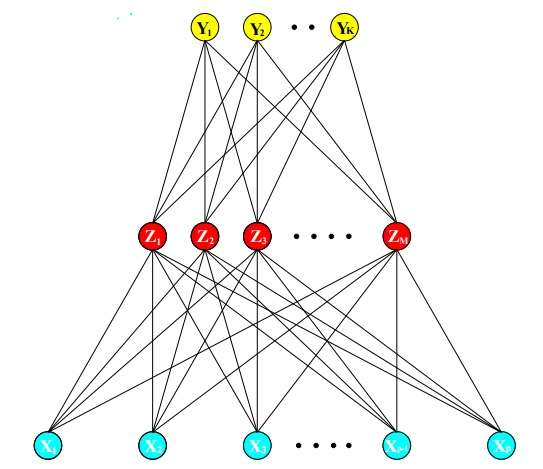
\includegraphics[width=\linewidth]{tg1/figuras/ANN.jpeg}
% 		\caption{Perceptron de Várias Camadas ou MLP \cite{hastie_09_elements-of.statistical-learning}} \label{fig:ANN}
% 	\end{minipage}
% \end{figure}


% \todo{tirar essa parte falando de MLP e RF???}

% Também é frequente utilizar um modelo conhecido como \textit{Random Forest}, um modelo \textit{ensemble}, isto é, um algoritmo que emprega várias cópias do mesmo modelo operando em paralelo. O \textit{Random Forest} produz várias árvores de decisão independentes que processam os dados fornecidos e produzem um resultado final, isto é, cada árvore faz sua classificação ou regressão. A partir disso, o resultado final é decidido por meio de uma "eleição" entre a saída de todas as árvores. Este modelo é bastante empregado para algumas situações por demonstrar bons resultados a partir de dados categóricos, além de ser bem fácil de ser visualizado e interpretado por ser semelhante a uma árvore de cabeça para baixo \cite{oreillyML}

\subsection{\textbf{Função de Custo}}

Todo modelo de aprendizado de máquina faz uso de uma função de custou ou função de erro. Este termo se trata de uma equação que computa a diferença entre a saída do modelo e o resultado esperado, e a partir deste valor os parâmetros do modelo são ajustados de forma a minimizar esta função. 

Utilizando uma linguagem mais matemática, uma estratégia comum de se encontrar um mínimo de uma função se da pelo uso de sua derivada, que fornece o ângulo da curva função em um dado ponto. Ou seja, a partir disto é possível incrementar a função em pequenos valores, encaminhando-a a uma direção onde sua derivada seja nula, isto é, um ponto mínimo. Esta técnica é conhecida como \textit{Gradient Descent} \cite{cauchy}, ou Gradiente Descendente. 



% A situação ideal no treinamento de um modelo é que este atinja um mínimo global, um ponto menor do que todos os outros pontos vizinhos na função de custo. Porém, normalmente se atinge um mínimo local, um ponto que é o menor dentro de sua vizinhança imediata. Isso pode sinalizar o fim do Gradiente Descendente e encerrar o aprendizado em um ponto diferente mínimo global. Em outras palavras, o modelo não minimizou a função da melhor forma possível \cite{GoodBengCour16}.

\subsection{\textbf{Dataset}}
\label{dataset}

O conjunto de dados é vital para o funcionamento do algoritmo de aprendizado. Em geral, o primeiro passo no desenvolvimento de um algoritmo de aprendizado de máquina é a criação de um \textit{Dataset}. Para um modelo tabular, os dados são dispostos na forma de uma tabela enquanto para um modelo convolucional, os dados são fornecidos na forma de imagens. De qualquer forma, uma quantidade suficiente de dados é necessária para um bom treinamento do modelo.

Os dados normalmente são separados em conjuntos de dados de Treinamento e dados de Validação. Dados de treinamento são auto explicativos, isto é, são utilizado para treinar o modelo, enquanto dados de validação são utilizados rotineiramente no treinamento para se checar a acurácia do modelo com um conjunto de dados diferente do utilizado no treinamento. Também é comum de se utilizar um terceiro conjunto, um conjunto de Teste onde o modelo com treinamento concluído processa um novo conjunto diferente para fins de métricas de performance.

%Na internet é possível encontrar vários conjuntos de dados públicos. Um \textit{Dataset} bastante conhecido se chama \textit{MNIST Database} \cite{lecun-mnisthandwrittendigit-2010}, que contém diversas imagens de dígitos manuscritos utilizado para treinar modelos de reconhecimento de escrita por imagens. \todo{é relevante?^^} 
%\todo{falar de serie temporal, redes recorrentes}

\subsubsection{\textbf{Série Temporal}}
Um conjunto de dados de série temporal (ou "dataset" de série temporal) é uma coleção de informações organizadas de maneira sequencial, onde cada ponto de dados está associado a um período de tempo específico. Esse tipo de conjunto de dados é usado para registrar observações, medições ou valores ao longo do tempo. 
Os datasets de séries temporais são frequentemente usados em análises estatísticas, modelagem preditiva e aprendizado de máquina para entender tendências, padrões sazonais e comportamentos ao longo do tempo.

\subsubsection{\textbf{Normalização do \textit{Dataset}}}

Normalizar os dados é uma etapa crucial de pré-processamento que consiste em ajustar as características para uma faixa comum, evitando que valores numericamente mais elevados de algumas características dominem sobre os valores numericamente menores. O principal propósito é reduzir o viés daquelas características cuja contribuição numérica é mais significativa na distinção entre as classes \cite{SINGH2020105524}.

\subsection{\textbf{\textit{Overfitting}}}

\textit{Overfitting}, ou sobreajuste em português, ocorre quando um modelo de machine learning se ajusta excessivamente aos dados de treinamento de maneira que ele passe a falsa impressão de que possui um alto rendimento, porém ao receber dados novos de entrada, a precisão da saída cai consideravelmente \cite{overftt}.

\begin{figure}[htb]
	\centering
	\begin{minipage}{0.9\linewidth}
		\centering
		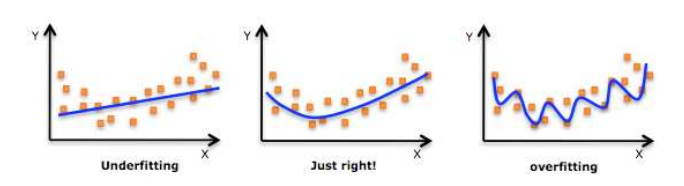
\includegraphics[width=\linewidth]{tg1/figuras/overfiting.png}
		\caption{
            \cite{overftt}} \label{fig:overftt}
	\end{minipage}
\end{figure}

Na imagem \ref{fig:overftt} temos um exemplo de sobreajuste para um modelo de regressão, podemos deduzir do gráfico que a função encontrada é a que melhor minimiza a função de erro do modelo, porém ela certamente não é capaz de ser generalizada para novos dados.

O \textit{overfitting} ocorre quando um modelo é treinado excessivamente nos dados de treinamento, capturando padrões específicos desses dados que não são generalizáveis para novos dados. O modelo acaba por incorporar o ruído dos dados de entrada, levando a previsões imprecisas quando o modelo é exposto a novos dados com ruído diferente.

\subsection{\textbf{Métricas de Avaliação do Modelo}}

A avaliação de modelos de aprendizado de máquina é crucial para desenvolver um bom algoritmo de aprendizado de máquina. Métricas de avaliação fornecem uma medida objetiva do desempenho do modelo, permitindo comparações entre diferentes abordagens.

Métricas são essenciais no ajuste fino dos hiper parâmetros do modelo de aprendizado de máquina. A partir deles, é possível diagnosticar problemas como \textit{overfitting} ou explosão de gradiente. Os dados gerados são acurácia, precisão, \textit{recall} e \textit{f-score} para cada classe e no total de forma ponderada. Além disso também são registrados os valores dos pesos dos nós da rede neural de forma a se observar explosões ou desaparecimentos de gradiente.

\begin{figure}[ht]
    \text{Acurácia} = $\frac{\text{Número de previsões corretas}}{\text{Número total de previsões}}$
    \centering
    \caption{Fórmula para \textbf{acurácia}}
\end{figure}

\begin{figure}[ht]
    \[\text{Precisão} = \frac{tp}{tp+fp}\]
    \centering
    \caption{Fórmula para \textbf{precisão}}
\end{figure}


\begin{figure}[ht]
    \[F_{1} = \frac{2tp}{2tp + fp + fn}\]
    \caption{Fórmula para \textit{F-score}}
\end{figure}

\begin{figure}[ht]
    \[ \textit{recall} =  \frac{tp}{tp + fn}\]
    \caption{Fórmula para \textit{recall}}
\end{figure}

Onde "tp" é quantidade de verdadeiros positivos, "fp" falsos positivos e "fn" falsos negativos. \textit{F-score} é uma métrica útil para medir o aprendizado da rede pois é uma forma de levar em consideração o desequilíbrio entre classes. Por exemplo, em uma tarefa de classificação cujo a classe 1 representa apenas 1\% dos dados teria uma acurácia de 99\% caso exibisse apenas a classe 0 como resultado, porém o \textit{F-score} traria um resultado péssimo, informando a falha da rede. Já o \textit{recall}, que é utilizado no cálculo do \textit{F-score}, mede a capacidade de um modelo identificar corretamente todos os exemplos positivos em um conjunto de dados.

\section{Modelos de aprendizado de máquina}

\subsection{\textbf{\textit{Random Forest}}}

Um modelo \textit{ensemble}, isto é, um algoritmo que emprega várias cópias do mesmo modelo operando em paralelo. O \textit{Random Forest} produz várias árvores de decisão independentes que processam os dados fornecidos e produzem um resultado final, isto é, cada árvore faz sua classificação ou regressão. A partir disso, o resultado final é decidido por meio de uma "eleição" entre
a saída de todas as árvores. Este modelo é bastante empregado para algumas situações por demonstrar bons resultados a partir de dados categóricos, além de ser bem fácil de ser visualizado e interpretado por ser semelhante a uma árvore de cabeça para baixo \cite{oreillyML}.

Cada árvore de decisão é construída dividindo os dados em nós de decisão com base em características específicas. A seleção das características é feita de forma aleatória, o que impede que uma árvore dependa excessivamente de uma única característica, tornando o modelo mais robusto.

\begin{figure}[htb]
	\centering
	\begin{minipage}{0.9\linewidth}
		\centering
		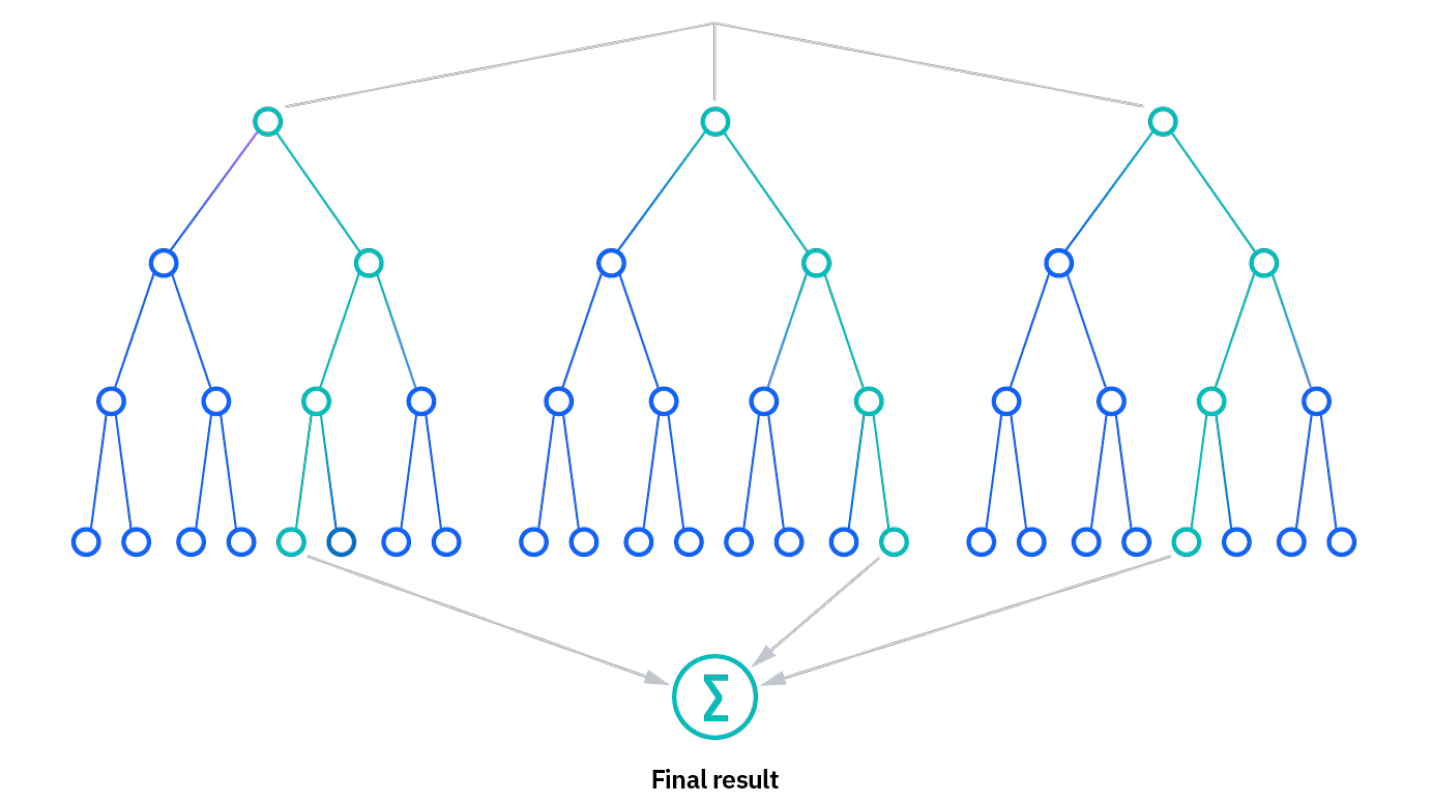
\includegraphics[width=\linewidth]{tg1/figuras/random.png}
		\caption{Ilustração exemplo de um modelo Random Forest
            \cite{rf_fig}} \label{fig:rfmodel}
	\end{minipage}
\end{figure}

\subsection{\textbf{MLP (\textit{MutiLayer Perceptron)}}}

Caracterizado por camadas com vários nós, semelhantes a neurônios,
com conexões entre si, semelhantes às sinapses. É o modelo mais comum das tais Redes Neurais, apresentando uma camada de entrada (Input Layer) e saída (Output Layer) e um número qualquer de camadas invisíveis (Hidden Layer) entre ambas \cite{hastie_09_elements-of.statistical-learning}.

Cada "neurônio" do MLP processa uma combinação linear das saídas da camada anterior por meio de pesos (Weights), aplica uma função de ativação não linear (Activation Function), e passa o resultado para os neurônios na próxima camada.

\begin{figure}[H]
	\centering
	\begin{minipage}{0.9\linewidth}
		\centering
		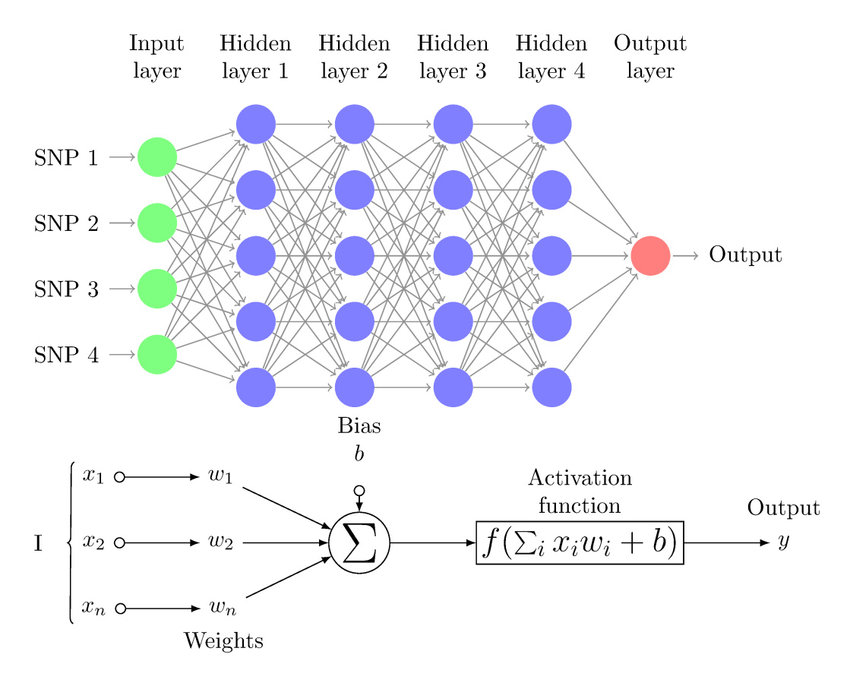
\includegraphics[width=\linewidth]{tg1/figuras/Multi-Layer-Perceptron-MLP-diagram-with-four-hidden-layers-and-a-collection-of-single.png}
		\caption{Ilustração exemplo de um modelo MLP
            \cite{mlp_fig}} \label{fig:mlpmodel}
	\end{minipage}
\end{figure}

\subsection{\textbf{LSTM (\textit{Long Short-Term Memory) }}}

LSTM (\textit{Long Short-Term Memory}) é um tipo de arquitetura de rede neural recorrente (RNN) que é projetada para lidar com sequências de dados e é especialmente eficaz em capturar dependências de longo prazo em sequências temporais \cite{lstm-}. Sua característica fundamental é a capacidade de "lembrar" informações importantes de longo prazo enquanto processam sequências de dados. Isso é alcançado por meio de unidades de memória especiais chamadas células de memória.

\begin{itemize}
    \item Porta de Esquecimento (Forget Gate): Esta porta decide quais informações da célula de memória anterior devem ser esquecidas ou mantidas com base no conteúdo atual da sequência. Ela ajuda a lidar com a questão do esquecimento de informações em sequências longas.
    
    \item Porta de Entrada (Input Gate): A porta de entrada permite que novas informações sejam adicionadas à célula de memória com base na sequência atual. Ela decide quais informações são relevantes para adicionar.
    
    \item Porta de Saída (Output Gate): A porta de saída determina qual parte da célula de memória será a saída da LSTM com base no conteúdo atual da sequência.
    
\end{itemize}

Em questões práticas, a rede neural LSTM recebe três entradas: \textit{cell state} ou estado de célula, \textit{hidden state} ou estado oculto e os dados de entrada. A entrada \textit{cell state} é projetada para capturar dependências de longo prazo em sequências, armazenando e transportando informações relevantes ao longo do tempo e é alterada pelas três portas da rede. Já a \textit{hidden state} é uma representação resumida das informações e pode ser usado como saída da LSTM ou alimentado às camadas subsequentes.

Esta arquitetura de rede neural foi projetada para lidar problemas comuns em redes recorrentes, a explosão ou o desaparecimento do gradiente, a partir do uso das portas e células de memória. Trata-se de uma rede com a capacidade de separar informações irrelevantes, permitindo com que o gradiente não varie caso não seja necessário.

\begin{figure}[htb]
	\centering
	\begin{minipage}{0.7\linewidth}
		\centering
		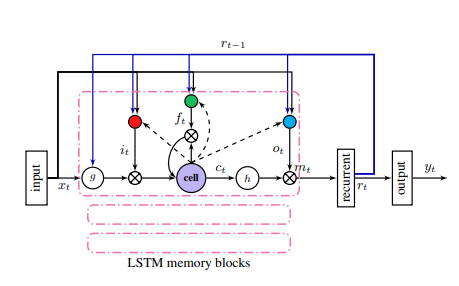
\includegraphics[width=\linewidth]{tg1/figuras/lstm.png}
		\caption{Ilustração exemplo de uma célula de um modelo LSTM
            \cite{lstm_fig}} \label{fig:lstmcell}
	\end{minipage}
\end{figure}

\begin{figure}[htb]
	\centering
	\begin{minipage}{0.6\linewidth}
		\centering
		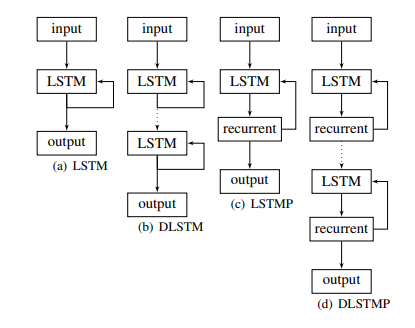
\includegraphics[width=\linewidth]{tg1/figuras/lstm_arch.png}
		\caption{Possíveis arquiteturas com LSTM
            \cite{lstm_fig}} \label{fig:lstmarch}
	\end{minipage}
\end{figure}

\todo{procurar imagens diferentes}



\section{Evento de Fogo}

Os Eventos de Fogo podem ser acessados por meio do Painel do Fogo \cite{painel-fogo}, uma plataforma gerida pelo Censipam \cite{censipam}. Este órgão é subordinado ao ministério da defesa e é responsável por articular ações de governo em prol da proteção ambiental e do desenvolvimento sustentável da Amazônia Legal e da Amazônia Azul.

Os eventos são gerados a partir de observações dos sensores orbitais VIIRS, por meio dos satélites NOAA-20 e SUOMI NPP, e MODIS, por meio dos satélites Aqua e Terra. Estes sensores detectam fogos ativos, formando uma camada vetorial. Em outras palavras, eventos detectados delimitam uma região e quando esta se intersecta com outra durante a mesma passagem do satélite, é gerado um vetor, polígono, que contém todos os eventos detectados na vizinhança e sua evolução ao longo do tempo.


\section{Tipificação do Fogo}

A tipificação do fogo se trata de uma classificação de um evento de incêndio que leva em consideração de diversas condições e características ambientais de forma a classificar o incêndio floresto na região amazônica entre quatro tipos:

\begin{itemize}
    \item \textbf{Savana e pastagem}:  Em regiões onde a vegetação natural é composta principalmente de savana, cerrado ou pastagens, os incêndios frequentemente ocorrem durante a estação seca devido à combinação de condições climáticas secas e atividade humana, como a queima de pastagens para melhorar o crescimento da grama. Vegetação de porte baixo, com pouca presença de biomassa, longa duração dias-semanas;
    \item \textbf{Pequenas clareiras}: Esse tipo de incêndio ocorre em áreas florestais onde as árvores foram cortadas recentemente, criando clareiras. O objetivo pode ser a remoção de resíduos de madeira ou a preparação do solo para o plantio. Pequenos incêndios em sistemas florestais (cobertura de árvores > 50$\%$ e igual ou inferior a 5 detecções de incêndios), curta duração, área menor que 100 ha;
    \item \textbf{Sub-bosque}: Os incêndios no sub-bosque ocorrem em florestas maduras, onde o fogo queima principalmente sob a copa das árvores, afetando a vegetação e o solo abaixo da copa das árvores. Esses incêndios podem ser causados por raios, atividades humanas ou ser usados como ferramenta de manejo florestal. Vegetação de porte arbustivo alto, Apresenta altas taxas de biomassa. Ocorre muito em borda de áreas desmatadas com floresta. Área variável, longa duração, poucos focos de calor por detecção, mesma região geográfica do desmatamento;
    \item \textbf{Desmatamento}: Esses incêndios ocorrem principalmente devido à atividade humana, como a conversão de áreas florestais em terrenos agrícolas, pastagens ou áreas urbanas. São frequentemente associados ao desmatamento ilegal. Os incêndios de desmatamento normalmente têm alto poder radiativo inicial do fogo, pois os detritos lenhosos empilhados levam a uma maior liberação de energia e longa persistência do fogo, uma vez que essas pilhas podem arder por dias. Maior poder radiativo no início, maior duração, área variável.

\end{itemize} 

Os dados necessários para esta classificação são relativos à vegetação (como biomassa e cobertura) e características do incêndio (como persistência e tamanho) \cite{gfed}.

%\begin{mdframed}[style=defnSty] % azul
%\begin{mdframed}[style=plainSty] % verde

%{\center \textsc{Texto motivador} \par}

%\noindent Esperamos que o \abnTeX\ aprimore a qualidade do trabalho que você produzirá, de modo que o principal esforço seja concentrado no principal: na contribuição científica.
   
%\end{mdframed}